%%%%%%%%%%%%%%%%%%%%%%%%%%%%%%%%%%%%%%%%%%%%%%%%%%%%%%%%%%


% Poggendorff Illusion in TikZ
% https://latexdraw.com
% 21/12/2020, 19:13

\documentclass[border=0.2cm]{standalone}

\usepackage{tikz}

\begin{document}


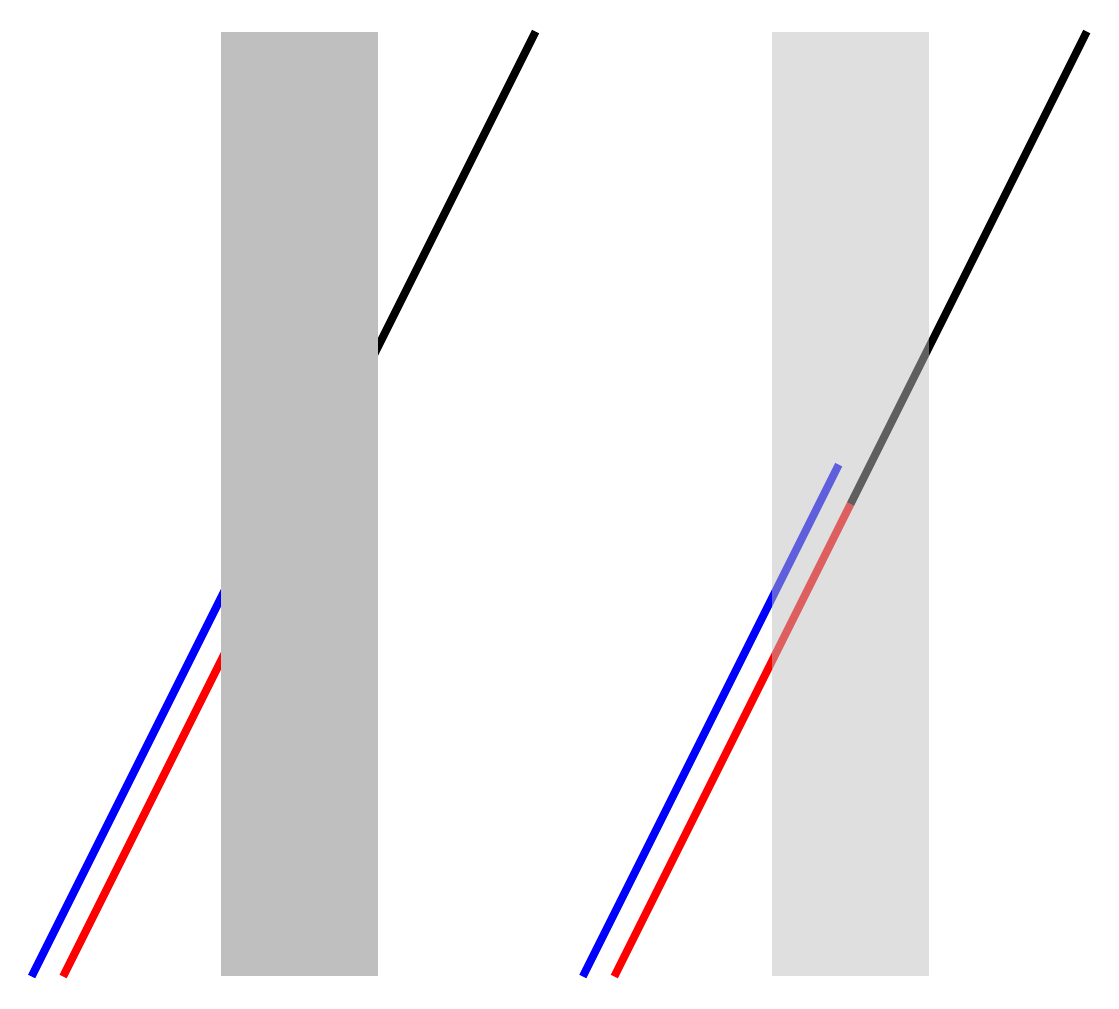
\begin{tikzpicture}

% Left side illustration

\draw [line width=1mm,red] (0,0) -- ++ (3,6);
\draw [line width=1mm,black] (3,6) -- ++ (3,6);
\draw [line width=1mm,blue] (-0.4,0) -- ++ (3.25,6.5);

% rectangle
\fill[lightgray] (2,0) rectangle ++(2,12);

% Right side illustration

\begin{scope}[xshift=7cm]
\draw [line width=1mm,red] (0,0) -- ++ (3,6);
\draw [line width=1mm,black] (3,6) -- ++ (3,6);
\draw [line width=1mm,blue] (-0.4,0) -- ++ (3.25,6.5);

% rectangle
\fill[lightgray,opacity=0.5] (2,0) rectangle ++(2,12);
\end{scope}

\end{tikzpicture}

\end{document}
